\subsection{Interaction viewpoint}
    

    \subsubsection{Looping System UML sequence diagram}
        \begin{figure}[!ht]
            \centering
            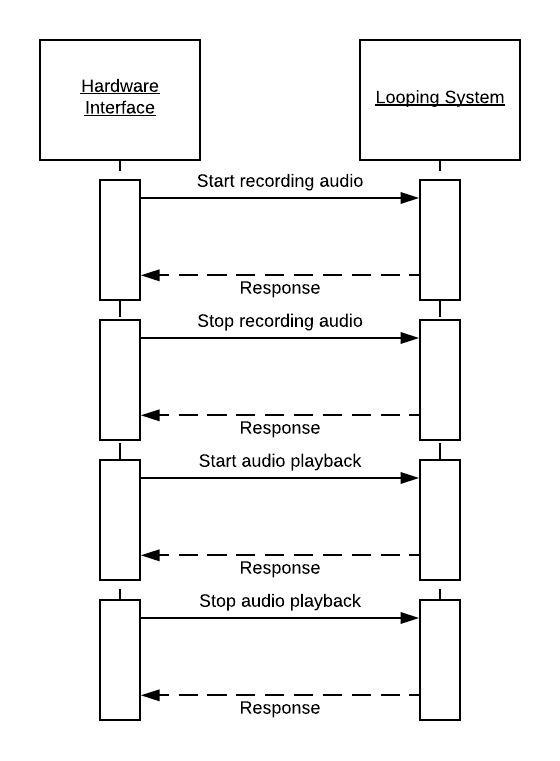
\includegraphics{diagrams/looping-interaction.jpeg}
            \caption{Looping System sequence diagram}
            \label{fig:looping}
        \end{figure}
       Figure \ref{fig:looping} shows the intended interaction of the Hardware Interface and Looping Subsystem. Physical controls on the Hardware Interface correspond directly to the functionality of the Looping system. Creating a one to one relationship between the physical controls on the hardware and the software functionality they control should facilitate intuitive control while affecting the Looping System.
       
    \subsubsection{Audio Modulation System UML sequence diagram}
        \begin{figure}[!ht]
            \centering
            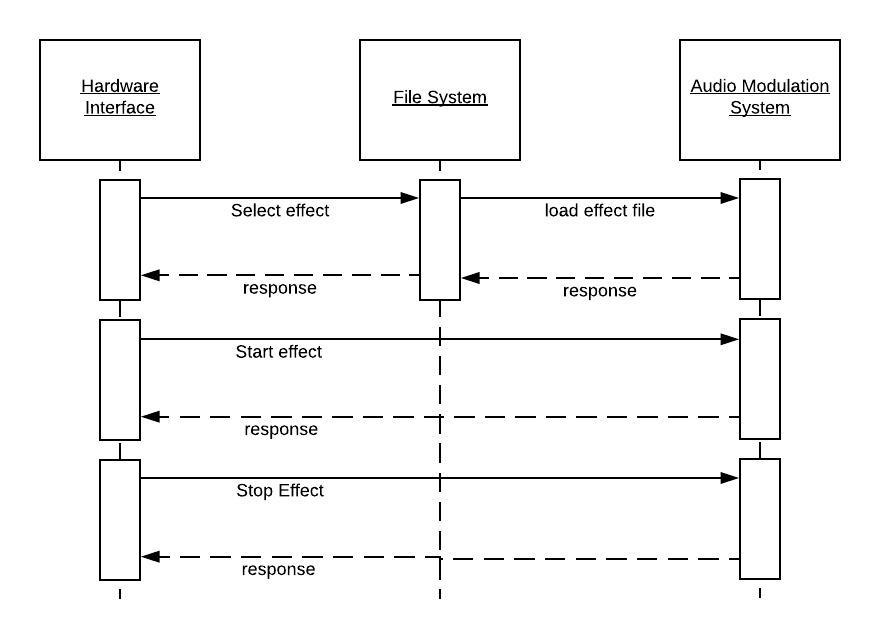
\includegraphics{diagrams/modulation-interaction.jpeg}
            \caption{Audio Modulation System sequence diagram}
            \label{fig:modulation}
        \end{figure}
        Figure \ref{fig:modulation} illustrates the intended interaction between the Hardware Interface and the Audio Modulation System.
        